%*******************************************************************************
% Definicje stylu dokumentu
%*******************************************************************************

%===============================================================================
% klasa dokumentu

%\documentclass[12pt, a4paper, twoside, titlepage, final]{mwbk}
\documentclass[10pt,a4paper,onecolumn,twoside,11pt,wide,floatssmall]{book}
%\documentclass[10pt,a4paper,onecolumn,oneside,11pt,wide,floatssmall]{article}


%===============================================================================
% Pakiety
%\usepackage[latin2]{inputenc}
\usepackage{polski}
%\usepackage[cp1250]{inputenc}
\usepackage[utf8]{inputenc}				% kodowanie �r�d�a
\usepackage[polish]{babel}				% polskie przenoszenie wyraz�w (hyph.)
\usepackage[T1]{fontenc}					% font PL
\usepackage{url}								% polecenie \url
\usepackage{amsfonts}						% fonty matematyczne
\usepackage{graphicx}						% wstawianie grafiki
\usepackage{color}							% kolory
\usepackage{fancyhdr}						% paginy g�rne i dolne
\usepackage[plainpages=false]{hyperref}		% dynamiczne linki
\usepackage{calc}							% operacje arytmetyczne w TeX'u
\usepackage{tabularx}						% rozci�gliwe tabele
\usepackage{array}							% standardowe tabele
\usepackage{geometry}
\usepackage{hyperref}
\usepackage{subfigure}
\usepackage{wrapfig}
\usepackage{indentfirst}
\usepackage{amsmath}
\usepackage{color}
\usepackage{array}
\usepackage{pdflscape}
\usepackage{amsmath}
\usepackage{textcomp}
\usepackage[font={small,it}]{caption}
\usepackage{etoolbox}
\usepackage[section]{placeins}
\usepackage{float}
\graphicspath{{./img/}}
\usepackage{listings}             % Include the listings-package
\usepackage{enumitem}


\linespread{1.3}								% 1.3 do interlinii 1.5


\patchcmd{\thebibliography}{\chapter*}{\section*}{}{}

\bibliographystyle{plain}
% w�asne pakiety

%===============================================================================
% Ustawienia dokumentu

\frenchspacing

% ustawienia wymiar�w
\oddsidemargin 0mm							% margines nieparzystych stron
\evensidemargin 0mm							% margines parzystych stron
\headheight 15pt								% wysoko�� paginy g�rnej
\topmargin 0mm									% margines g�rny
\setlength{\parindent}{0pt}
\setlength{\parskip}{1ex plus 0.5ex minus 0.2ex}
% styl paginacji
\pagestyle{fancy}
% \renewcommand{\chaptermark}[1]{}%{\markboth{#1}{}} % BO ARTICLE
\renewcommand{\sectionmark}[1]{}%{\markright{\thesection\ #1}{}}
\renewcommand{\thesection}{\arabic{section}}


% nag��wek 
\fancyhf{}

\fancyhead[RE,LO]{\thepage}
\fancyhead[LE,RO]{[GIS]~Teoria grafów w modelowaniu epidemii}
\renewcommand{\headrulewidth}{0.1pt}
\renewcommand{\footrulewidth}{0pt}

% nag��wek w stylu plain 
\fancypagestyle{plain}
{
\fancyhf{}
\renewcommand{\headrulewidth}{0pt}
\renewcommand{\footrulewidth}{0pt}
}

% ta sekwencja tworzy czyste kartki na stronach po \cleardoublepage
\makeatletter
\def\cleardoublepage{\clearpage\if@twoside \ifodd\c@page\else
	\hbox{}
	\vspace*{\fill}
	\thispagestyle{empty}
	\newpage
	\if@twocolumn\hbox{}\newpage\fi\fi\fi}
\makeatother

%===============================================================================
% Zmienne �rodowiskowe i polecenia

% definicja
% \newtheorem{definition}{Definicja}[chapter] % BO CHAPTER
\newtheorem{definition}{Definicja}

% twierdzenie
% \newtheorem{theorem}{Twierdzenie}[chapter] % BO CHAPTER
\newtheorem{theorem}{Twierdzenie}

% obcoj�zyczne nazwy
\newcommand{\foreign}[1]{\emph{#1}}

% pozioma linia
\newcommand{\horline}{\noindent\rule{\textwidth}{0.4mm}}

% wstawianie obrazk�w {plik}{caption}{opis}
\newcommand{\fig}[3]
{
\begin{figure}[!htb]
\begin{center}
\includegraphics[width=\textwidth]{#1}
\caption[#2]{#2. #3}
\label{#1}
\end{center}
\end{figure}
}

%===============================================================================
% ustawienia pakietu hyperref

\hypersetup
{
%colorlinks=true,			% false: boxed links; true: colored links
%linkcolor=black,			% color of internal links
%citecolor=black,			% color of links to bibliography
%filecolor=black,			% color of file links
%urlcolor=black			% color of external links
}

%===============================================================================

% Custom titlepage
\makeatletter
\newcommand*{\subtitle}[1]{\newcommand*{\@subtitle}{#1}}
\newcommand*{\supervisor}[1]{\newcommand*{\@supervisor}{#1}}
\newcommand*{\course}[1]{\newcommand*{\@course}{#1}}
\newcommand*{\coursecode}[1]{\newcommand{\@coursecode}{#1}}
\newcommand*{\university}[1]{\newcommand{\@university}{#1}}
\newcommand*{\faculty}[1]{\newcommand{\@faculty}{#1}}
\newcommand{\sepline}{\rule{\linewidth}{0.4mm}}
% ------------------------------------------------------------------------------ 
\renewcommand*{\maketitle}{%
	\@ifundefined{@course}{%
		\providecommand*{\@course}{\VariableNotSetFix{\course}}%
		
	}{}
	

	\hypersetup{pageanchor=false}
	\begin{titlepage}%
		\vspace*{1cm}
		
		\begin{figure}[H]
			\centering
			
\includegraphics[width=3cm]{weiti_logo.png} % Include a department/university logo - this will require the graphicx package
			\label{fig:logo}
		\end{figure}
		\begin{center}%
			\@ifundefined{@university}{}{%
				{\small \@university \par}}%
			\@ifundefined{@faculty}{}{%
				{\small \@faculty \par}}%
		\end{center}
		%\vspace{1cm}
		\begin{center}%
			\@ifundefined{@coursecode}{%
				{\Large \@course \par}%
			}{%
			{\Large \@course \ (\@coursecode) \par}}%
	\end{center}
	\sepline
	\begin{center}%
		{\LARGE \textsc{\@title} \par}
		\@ifundefined{@subtitle}{}%
		{\vspace{0.5cm}%
			\normalsize \textsc{\@subtitle} \par}%
	\end{center}
	\sepline
	\vspace{1cm}
	\begin{center}%
		{\normalsize
			\itshape
			\lineskip .5em%
			\begin{tabular}[t]{c}%
				\@author
			\end{tabular}\par}%
	\end{center}
	\vspace{2cm}
	\@ifundefined{@supervisor}{}{%	
		\begin{flushright}%
			{\normalsize Opiekun projektu: \par}
			{\normalsize \itshape \@supervisor \par}
		\end{flushright}		
		
	}
	%\vfill\null
	\begin{center}%
		\@date
	\end{center}
	
	\@thanks
\end{titlepage}%
\hypersetup{pageanchor=true}
\setcounter{footnote}{0}%
\global\let\thanks\relax
\global\let\maketitle\relax
\global\let\@thanks\@empty
\global\let\@author\@empty
\global\let\@date\@empty
\global\let\@title\@empty
\global\let\title\relax
\global\let\author\relax
\global\let\date\relax
\global\let\and\relax

}

\makeatother

\title{Teoria grafów w~modelowaniu epidemii}
\subtitle{Sprawozdanie 3}
\author{%
	Michał Dobrzański\\
	\texttt{\href{mailto:mdobrzan@mion.elka.pw.edu.pl}%
		{\nolinkurl{mdobrzan@mion.elka.pw.edu.pl}}}
	\and
	Maciej Janusz Krajsman\\
	\texttt{\href{mailto:M.Krajsman@stud.elka.pw.edu.pl}%
		{\nolinkurl{M.Krajsman@stud.elka.pw.edu.pl}}}
}
\supervisor{mgr inż. Łukasz Błaszczyk}
\university{Politechnika Warszawska}
\faculty{Wydział Elektroniki i~Technik Informacyjnych}
\course{Grafy i~Sieci}
\coursecode{GIS}

\begin{document}
\lstset{language=Python} 

\maketitle
\tableofcontents
\clearpage

\section{Szczegółowy opis merytoryczny zadania}
\label{sec:szczegolowy_opis_merytoryczny_zadania}

Zadaniem projektowym jest \textbf{zaimplementowanie modelu SIS} rozwoju epidemii, zbadanie jego właściwości na grafach modelujących populację ludzi, w~których wierzchołek odpowiada konkretnej osobie. Należy również porównać otrzymane wyniki z~modelem ciągłym dla epidemii opisanym równaniami różniczkowymi.  

Zadanie będzie polegało na \textbf{wygenerowaniu odpowiednich grafów losowych}, a~następnie na uruchomieniu \textbf{algorytmu propagacji epidemii} (zgodnego z~modelem SIS) dla wierzchołków tych grafów.

Otrzymane wyniki zostaną zestawione z~wynikami otrzymanymi za pomocą równań różniczkowych. Dla przejrzystości utworzone zostaną wykresy porównujące oba podejścia. Dobór prezentowanych parametrów dla osi wykresów zostanie określony w~trakcie tworzenia projektu.


\section{Opis algorytmu generowania grafów losowych według modelu sieci Barabásiego-Alberta}
\label{sec:opis_alg_ba}

Do zrealizowania projektu potrzebny będzie algorytm generujący grafy losowe według \textbf{modelu sieci Barabásiego-Alberta}. Utworzone sieci dzięki temu modelowi są nazywane sieciami przypadkowymi ewoluującymi.

Zaproponowana przez autorów \textbf{ewolucja sieci} rozumiana jako zmiany struktury sieci w~kolejnych odstępach czasowych modelowana jest poprzez dołączanie nowych węzłów do istniejącej już sieci. 

Procedura konstruowania sieci Barabásiego-Alberta obejmuje następujące kroki:

\begin{enumerate}
\item Na początkowym etapie ewolucji (czyli w~chwili $t = 0$) siecią nazywamy graf pełny (całkowicie połączony klaster węzłów) o~rozmiarze: $m_0 >= 1$. W~następnych krokach czasowych $t = 1,2,3,...$ do sieci dodawane są nowe węzły (jeden węzeł na jeden krok), które tworzą odpowiednio $m <= m_0  (m = const)$ połączeń (czyli krawędzi) do istniejących już wierzchołków sieci.
\item Proces dodawania wierzchołków realizuje \textbf{regułę preferencyjnego dołączania}, która mówi o~tym, że prawdopodobieństwo, że nowy wierzchołek utworzy połączenie do jednego ze starszych wierzchołków jest wprost proporcjonalne do stopnia wierzchołka starszego.
\item Wzrost sieci kończony jest w~dowolnej chwili t. W~momencie zakończenia wzrostu sieć ma $N$ wierzchołków (węzłów) oraz $E$ (równanie \ref{eq:wierzch_ba}) krawędzi (równanie \ref{eq:kraw_ba}).
\begin{equation}
\label{eq:wierzch_ba}
N = t + m_0 \approx t
\end{equation}
\begin{equation}
\label{eq:kraw_ba}
E = mt + \binom{m_0}{2} \approx mt
\end{equation}
\end{enumerate}


\section{Szczegółowy opis modelu SIS rozwoju epidemii}
\label{sec:szczegolowy_opis_modelu_sis_rozwoju_epidemii}

\textbf{Model SIS} opiera się na zestawie równań różniczkowych, które opisują \textbf{rozprzestrzenianie się chorób zakaźnych}. Służy do określania, czy dana choroba \textbf{zaniknie}, czy \textbf{ustali się} na konkretnym poziomie. Jest najbardziej ogólnym modelem matematycznym tego zjawiska --- nie uwzględnia np. przypadków nosicielstwa i~uodpornienia, istnienia osobników w~fazie utajonej choroby czy urodzeń chorych. Stan populacji w~tym modelu opisany jest \textbf{tylko jedną zmienną (\textit{I})}, która reprezentuje liczbę osobników zainfekowanych.

\subsection{Założenia modelu SIS}
\label{subsec:zalozenia_modelu_sis}

\begin{description} \itemsep0pt
\item[$\bullet$] Jednostki mogą znajdować się w~jednym z~dwóch stanów:
  \begin{description} \itemsep0pt
  \item[S] \textit{(susceptible --- ang. podatni)} --- jednostki są zdrowe, podatne na zakażenie.
  \item[I] \textit{(infected --- ang. zainfekowani)} --- jednostki są chore, mogą zakażać zdrowe jednostki.
  \end{description}
\item[S(t)] --- liczba osobników podatnych (zdrowych), tj. liczba węzłów w~stanie S~w~danej chwili czasowej $t$.
\item[I(t)] --- liczba jednostek zainfekowanych, tj. liczba węzłów w~stanie I~w~danej chwili czasowej $t$.
\item[$\bullet$] Do zakażenia (zmiany stanu węzła z~$S$ na $I$ może dojść na skutek kontaktu jednostki zdrowej i~chorej.
\item[N] --- liczebność populacji, dla której $N = S(t) + I(t)$, Liczebność populacji jest stała, tj. $N = \textit{const.}$

\item[$\pmb{\beta}$] --- prawdopodobieństwo, że w~pojedynczym kroku czasowym ($dt$) zdrowy osobnik zostanie zakażony przez chorego sąsiada.
\item[$\pmb{\gamma}$] --- prawdopodobieństwo, że w~pojedynczym kroku czasowym ($dt$) chory osobnik wyzdrowieje, tj. zmieni stan $ I~\rightarrow S~$.
\item[$\pmb{\lambda}$] --- parametr określający \textbf{tempo rozprzestrzeniania się epidemii}. Jest to stosunek $\lambda = \beta / \gamma $.
\item[$\pmb{\lambda_c}$] --- \textbf{wartość progowa tempa rozprzestrzeniania się epidemii}. Gdy tempo przekroczy tą wartość krytyczną, wówczas epidemia ma szansę stać się powszechną, a~badana choroba nabrać charakteru endemicznego. Dla symulacji w~czasie nieograniczonym oznacza to endemię.

\end{description}


\subsection{Warunki początkowe}
\label{subsec:warunki_poczatkowe}

Dla sieci losowych oraz bezskalowych (BA) dzięki modelowi SIS można opisać propagację epidemii za pomocą równania różniczkowego określającego tempo zmiany w~czasie liczby zakażonych węzłów o~zadanym stopniu k. W~tym celu należy określić \textbf{warunki początkowe} epidemii, czyli w~chwili $t = 0$. 

Określa się:
\begin{description} \itemsep0pt
\item[P(k)] --- rozkład stopni wierzchołków otrzymany po wygenerowaniu grafu BA dla wszystkich wartości $k$.
\item[$\pmb{\beta, \gamma}$] --- określone prawdopodobieństwa odpowiednio: zdrowy zostanie zakażony przez chorego, chory wyzdrowieje.
\item[$\pmb{I_k(0)}$] --- początkowa liczba zainfekowanych węzłów o~stopniu $k$.
\item[$\pmb{S_k(0)}$] --- początkowa liczba podatnych węzłów o~tym samym stopniu $k$.
\end{description}

Pytanie, jakie zadaje się przy modelowaniu epidemii najczęściej brzmi: Czy dla zadanych wartości parametrów $\beta$ i~$\lambda$ oraz dla zadanej początkowej liczby zainfekowanych osobników $i_0(0)$ infekcja rozprzestrzeni się czy nie?

Ponadto dla sieci bezskalowych szuka się wartości parametru $\lambda_c$, czyli progu od którego epidemia może stać się powszechna w~danej populacji.

\subsection{Równania różniczkowe opisujące model}
\label{subsec:rownania_rozniczkowe_opisujace_model}

Oprócz wcześniej wymienionych parametrów dla modelu SIS w~sieciach bezskalowych określa się prawdopodobieństwo, że dowolna krawędź grafu prowadzi do węzła, który przechowuje stan o~wartości ,,chory''.

\begin{equation}
\label{eq:q_i}
Q_I = \sum_{k} Q(k) i_k
\end{equation}
Gdzie:
\begin{description} \itemsep0pt
\item[k] --- stopień wierzchołka.
\item[$\pmb{Q_I}$] --- prawdopodobieństwo, że dowolna krawędź grafu prowadzi do węzła, który przechowuje stan o~wartości ,,chory''
\item[$\pmb{Q(k)}$] --- prawdopodobieństwo, że dowolna krawędź grafu prowadzi do węzła o~stopniu $k$, który przechowuje stan o~wartości ,,chory''.
\item[$\pmb{i_k}$] --- prawdopodobieństwo, że węzeł o~stopniu $k$ przechowuje stan o~wartości ,,chory''.
\end{description}

Wartość $Q(k)$ można dla danej sieci powiązań dla danej populacji wyliczyć z~następującego wzoru:
\begin{equation}
\label{eq:q_k}
Q(k) = \frac{k}{\langle k \rangle}P(k)
\end{equation}
Gdzie:
\begin{description} \itemsep0pt
\item[k] --- stopień wierzchołka.
\item[$\pmb{\langle k \rangle}$] --- gęstość sieci. Średni stopień losowo wybranego wierzchołka.
\end{description}

W przypadku sieci BA o~tworzeniu połączeń w~sieci nie decyduje żadne z~góry narzucone prawo, jej \textbf{struktura zależy od indywidualnych decyzji jej elementów} (kto kogo poznał, kto się z~kim widuje). W~rezultacie otrzymujemy \textbf{potęgowy rozkład stopni wierzchołków}, w~którym w~bliskim sąsiedztwie mogą występować wierzchołki o~ogromnej liczbie incydentnych krawędzi oraz te niemalże odizolowane od reszty sieci. Ze względu na potęgowy rozkład stopni wierzchołków, wyniki byłyby niewłaściwe. Równania korzystające ze średniego stopnia \emph{$\langle k \rangle$} ilustrują dynamikę układu zawierającego same wierzchołki o~średnim stopniu. W~opisie dynamiki sieci BA należy więc stosować równania dotyczące wierzchołków o~\textbf{zadanym stopniu \emph{k}}.

Tempo zmiany osobników zainfekowanych (węzłów o~zadanym stopniu $k$) $I_k(t)$ opisuje się następująco:

\begin{equation}
\label{eq:dii_k}
\frac{dI_k(t)}{dt} = [\beta k Q_I]S_k(t) - \gamma I_k(t)
\end{equation}

Można również wyliczać tempo zmiany prawdopodobieństwa, że konkretny osobnik (węzeł o~zadanym stopniu $k$) jest zainfekowany:
\begin{equation}
\label{eq:di_k}
\frac{di_k(t)}{dt} = [\beta k Q_I]s_k(t) - \gamma i_k(t);~~i_k(t) + s_k(t) = 1
\end{equation}
% Gdzie: $$
% \begin{itemize} \itemsep0pt
% \item 
% \end{itemize}

Szczególnie interesujący jest przypadek graniczny, dla $\displaystyle i_k =  \lim_{t\to\infty} i_k(t)$:
\begin{equation}
\label{eq:i_k_infty}
i_k = \frac{\lambda k Q_I}{1+\lambda k Q_I}
\end{equation}
Zgodnie z~zapisem w~sekcji \ref{subsec:zalozenia_modelu_sis}, parametr $\lambda = \beta / \gamma $ określa tempo rozprzestrzeniania się epidemii.
W powyższym równaniu (\ref{eq:i_k_infty}) określone zostało prawdopodobieństwo że węzeł o~stopniu \emph{k} jest w~stanie \emph{I} (jest zakażony) w~czasie nieskończonym, czyli po zakończeniu symulacji. Wyzerowanie $i_k$ zależy od $Q_I$, ponieważ \emph{k} jest dodatnią liczbą naturalną, a~$\lambda > 0$.
% Możemy dzięki temu stwierdzić, czy badana choroba utrzymuje się na stałym poziomie, czy zanika. 
By wykonywać obliczenia dla wszystkich stopni \emph{k}, należy zsumować obliczenia dla każdego z~nich. Z~wzorów (\ref{eq:q_i}), (\ref{eq:q_k}) i~ (\ref{eq:i_k_infty}) wynika, że:

\begin{equation}
\label{eq:q_i_expand}
Q_I = \sum_{k}Q(k)i_k = 1 - \frac{1}{\langle k \rangle}\sum_{k}P(k)\frac{k}{1+\lambda k Q_I} = f(Q_I)
\end{equation}
Gdzie:
\begin{description} \itemsep0pt
\item[k] --- stopień wierzchołka.
\item[$\pmb{f(Q_I)}$] --- funkcja rozkładu prawdopodobieństwa przechowywania stanu ,,chory'' przez węzły o~różnych stopniach.
\end{description}
Powyższe równanie może mieć jedno lub dwa rozwiązania. Jednym jest zawsze $Q_I = 0$ (dla $i_k = 0$). Obecność drugiego rozwiązania świadczy o~tym, że losowo wybrana krawędź prowadzi do zainfekowanego wierzchołka. Epidemia może się swobodnie rozwijać, więc $\lambda > \lambda_c$. Dzięki temu, warunek:

\begin{equation}
\label{eq:q_i_mt_one}
\left.\frac{df(Q_I)}{dQ_I}\right|_{Q_I=0} > 1
\end{equation}

umożliwia wyznaczenie $\lambda_c$. By funkcja (\ref{eq:q_i_expand}) spełniała warunek (\ref{eq:q_i_mt_one}):

\begin{equation}
\label{eq:q_i_mt_one_q_i}
\left.\frac{df(Q_I)}{dQ_I}\right|_{Q_I=0} = \left.\frac{1}{\langle k \rangle}\sum_{k}P(k)\frac{\lambda k^2}{(1+\lambda k Q_I)^2}\right|_{Q_I=0} = \frac{\lambda}{\langle k \rangle}\sum_{k}k^2P(k) = \lambda\frac{k^2}{k} > 1 
\end{equation}

Więc:
\begin{equation}
\label{eq:lambda_c}
\lambda_c = \frac{\langle k \rangle}{\langle k^2 \rangle}
\end{equation}


Okazuje się, że w~sieciach bezskalowych wartość parametru $\lambda_c$ jest bardzo zbliżona do zera. W~praktyce powinno to oznaczać, że powstrzymanie rozwoju epidemii jest prawie niewykonalne.


% \begin{equation}
% \label{eq:dSdt}
% \frac{dS}{dt} = -\frac{\beta SI}{N}+\mu(N-S)+\gamma I
% \end{equation}

% \begin{equation}
% \label{eq:dIdt}
% \frac{dI}{dt} = \frac{\beta SI}{N}-\gamma I-\mu I
% \end{equation}

% Gdzie ($\ref{eq:dSdt}$) określa tempo zmian liczebności grupy S~(zdrowych), a~($\ref{eq:dIdt}$) --- w~grupie I~(chorych).


\section{Opis planu zastosowania grafów losowych do omawianego zagadnienia}
\label{sec:opis_planu_zastosowania_grafow_losowych}

Wygenerowane grafy losowe według modelu Barabasiego-Arbert posłużą za model badanej populacji. \textbf{Wierzchołkami} będziemy reprezentowali poszczególne osoby w~danej populacji. \textbf{Krawędzie} będą przedstawiały natomiast relacje pomiędzy tymi osobami. Określamy, że dwa wierzchołki są sąsiednie, gdy mają wspólną krawędź grafu.

\textbf{Siecią losową, bezskalową} (w zadanej chwili $t$ utworzoną według modelu BA) będziemy nazywać określoną populację o~ustalonej liczności, która zostanie poddana modelowaniu zjawiska propagacji epidemii. 

Wierzchołki grafu będą przechowywały informacje o~stanie osoby --- czy jest ona zdrowa (podatna), czy chora (zakażająca) według modelu SIS. Zostanie zastosowana reprezentacja grafu za pomocą listy wierzchołków wraz z~odpowiadającymi im listami sąsiedztwa. Badanie rozwoju epidemii będzie bazowało na tej reprezentacji opisującej stan, w~jakim się dany graf znajduje.

\section{Podstawowe założenia implementowanego programu oraz projekt testów}
\label{sec:podstawowe_zalozenia_programu}

Program zostanie zaimplementowany w~środowisku Python. Do jego realizacji użyte zostaną biblioteki niezbędne do rysowania wykresów oraz grafów.

\textbf{Struktura grafu} będzie reprezentowana za pomocą listy sąsiedztwa. Dodatkowo w~niej dla każdego wierzchołka umieści się dodatkową informacją o~jego aktualnym stanie ($S$ lub $I$ według modelu SIS). W~środowisku Python będzie to słownik tworzony za pomocą konstruktora \textit{dict()}. Badanie algorytmu propagacji epidemii sprowadzi się do przechodzenia po listach sąsiedztwa i~zmianach stanów dla wierzchołków.

W implementowanym programie przeprowadzone zostaną następujące testy:
\begin{enumerate}
\item Sprawdzenie poprawności algorytmu generującego grafy losowe według modelu sieci Barabasiego-Alberta:

Zostaną wygenerowane sieci losowe BA (o różnych parametrach $m_0$, $m$ oraz $t$. Ich rozkłady stopni wierzchołków zostaną przedstawione na wykresie. Prawidłowo utworzone sieci według modelu BA powinny charakteryzować się w~przybliżeniu \textbf{potęgowym rozkładem stopnia wierzchołka}. Ten rozkład przybiera postać liniowego przebiegu na wykresie w~skali podwójnie logarytmicznej. Na tym wykresie wartość nachylenia krzywej przekłada się na wartość wykładnika dla rozkładu potęgowego. W~programie utworzony zostanie taki wykres i~przedstawione na nim będzie kilka przykładowych rozkładów dla różnych sieci losowych BA.

\item Przeprowadzenie symulacji rozwoju epidemii według modelu SIS dla różnych parametrów:

Następnie dla wcześniej wygenerowanych sieci losowych przeprowadzona zostanie symulacja rozwoju epidemii. Dla każdej sieci utworzone będzie kilka różnych warunków początkowych (odpowiednia liczba wierzchołków w~stanie $S$ i~$I$ w~chwili $t_0$, różne parametry $\gamma$, $\beta$). Następnie dla kolejnych chwil $t = 1,2,3,...$ będzie badany rozwój epidemii. Najistotniejszy jest wynik dla $t\to\infty$, ponieważ opisuje stan końcowy układu. Wyniki porównane zostaną ze spodziewanym rezultatem otrzymanym z~równań opisujących model SIS. Sprawdzone zostanie również, jak model zachowuje się dla $\lambda > \lambda_c$ oraz $\lambda < \lambda_c$ (w tym celu graf nie może być za mały, a~wartości $\lambda_c$ i~tak będą bardzo niewielkie, ze względu na potęgowy rozkład stopni wierzchołków grafu). 

\section{Opis kodu}
\label{sec:opis_kodu}

Zgodnie z~założeniami projektu, podstawowym zadaniem była grafowa implementacja modelu SIS. By sprawdzić, czy uzyskane wyniki są poprawne, zaimplementowano też rozwiązanie teoretyczne, na podstawie równań różniczkowych opisujących ten model. 

Zastosowane metody:
\begin{description}
\item[main()] --- Główna procedura, staruje kolejnością wykonywanych zadań i~parametrami pozostałych metod. Wypisuje część informacji w~konsoli.
\item[generate\_graph(m\_0, m, t)] --- Generuje graf Barabasiego-Alberta. Parametry: \emph{m\_0} --- liczba wierzchołków w~początkowym grafie pełnym, \emph{m} --- liczba krawędzi łączących każdy nowo dodany wierzchołek z~istniejącym wcześniej grafem, \emph{t} --- liczba wierzchołków do dodania w~procesie generowania grafu.
\item[pref\_addition(g, m)] --- Dodaje do grafu \emph{g} nowy wierzchołek, o~\emph{m} krawędziach incydentnych.
\item[get\_graph\_degree(g, print\_deg=False)] --- Zwraca rozkład stopni wierzchołków grafu \emph{g}. Parametr \emph{print\_deg} określa, czy wektor wynikowy będzie wypisany (\emph{True}) czy nie (\emph{False}).
\item[print\_graph(g)] --- Wypisuje graf \emph{g} w~konsoli, w~formacie:

\begin{lstlisting}[frame=single]
wierzcholek : [stan, [lista polaczen]]
\end{lstlisting}
np.
\begin{lstlisting}[frame=single]
1 : [0, [2, 3, 4, 6, 7, 10, 12, 20, 21, (...), 2989]]
\end{lstlisting}

\item[plot\_graph(g, $\pmb{(...)}$)] --- Rysuje graf \emph{g}. Pozostałe parametry określają wygląd grafu, są zgodne z~biblioteką \emph{matplotlib}.
\item[average\_graph\_degree(degrees, n\_graphs, m\_0, m, t)] --- Zwraca uśredniony rozkład stopni wierzchołków grafu, na podstawie wygenerowanych w~tym celu \emph{n\_graphs} grafów o~identycznych parametrach (\emph{m\_0}, \emph{m}, \emph{t}, zgodne z~\emph{generate\_graph(m\_0, m, t)}) jak początkowy graf.
\item[plot\_graph\_degree(g, m\_0, m, t, n\_graphs=5, alpha=3, ref\_length=0.8)] --- Rysuje rozkłady odniesienia oraz rozkład stopni wierzchołków w~grafie \emph{g} o~parametrach (\emph{m\_0}, \emph{m}, \emph{t}, zgodnych z~\emph{generate\_graph(m\_0, m, t)}). Parametr \emph{n\_graphs} określa, na podstawie ilu grafów tworzymy uśredniony rozkład. Parametry \emph{alpha} oraz \emph{ref\_length} służą do sterowania rozkładami odniesienia (pierwszy to współczynnik rozkładu potęgowego, drugi to względna długość rozkładów odniesienia).
\item[propagate\_sis(i\_k, beta, gamma, t\_max, degrees)] --- Teoretyczna implementacja modelu SIS na podstawie rozkładu prawdopodobieństwa zakażenia $i\_k$, w~przedziale czasowym $[0, t\_max]$. Parametry \emph{beta} oraz \emph{gamma} opisują model i~odpowiadają prawdopodobieństwom zakażenia i~wyzdrowienia. Wektor \emph{degrees} zawiera rozkład stopni wierzchołków w~modelu grafowym.
\item[infinite\_sis(i\_k, beta, gamma, degrees)] --- Oblicza rozwiązanie równania różniczkowego na podstawie rozkładu prawdopodobieństwa zakażenia $i\_k$, dla czasu dążącego do nieskończoności. Parametry \emph{beta} oraz \emph{gamma} opisują model i~odpowiadają prawdopodobieństwom zakażenia i~wyzdrowienia. Wektor \emph{degrees} zawiera rozkład stopni wierzchołków w~modelu grafowym.
\item[simulate\_sis(graph, beta, gamma, t\_max, degrees)] --- Grafowa implementacja modelu SIS dla grafu \emph{graph}, w~przedziale czasowym $[0, t\_max]$. Parametry \emph{beta} oraz \emph{gamma} opisują model i~odpowiadają prawdopodobieństwom zakażenia i~wyzdrowienia. Wektor \emph{degrees} zawiera rozkład stopni wierzchołków.
%\item[simulate\_average\_sis(graph, beta, gamma, t\_max, degrees, n\_sims=1)] --- Oblicza uśredniony wynik działania grafowej implementacji modelu SIS, na podstawie \emph{n\_sims} symulacji. Parametry symulacji \emph{graph}, \emph{beta}, \emph{gamma}, \emph{t\_max}, \emph{degrees}, zgodne z~\emph{simulate\_sis(graph, beta, gamma, t\_max, degrees)}
\item[calc\_q\_i(degrees,i\_k)] --- Oblicza wartość $Q_I$ na podstawie rozkładu stopni wierzchołków \emph{degrees} oraz rozkładu prawdopodobieństwa zakażenia \emph{i\_k}
\item[trim\_zeros(i\_k,degrees)] --- w~rozkładzie prawdopodobieństwa zakażenia $i_k$ zastępuje braki (dla rozkładu stopni wierzchołków \emph{degrees} nie występujących w~grafie) wartością \emph{-1}.
%\item[plot\_infected(t\_vec, infected\_number, infected\_max)] --- Rysuje wykres zależności liczby osobników chorych (\emph{infected\_number}) i~zdrowych (obliczana na podstawie liczby chorych) od chwili czasowej (\emph{t\_vec}). Parametr \emph{infected\_max} określa maksymalną liczbę osób zainfekowanych (czyli liczność populacji).
\item[plot\_sis(t, infected\_vect\_calc, infected\_vect\_sim, beta, gamma, k)] --- Rysuje wykres prawdopodobieństwa infekcji $i_k$ (dla wierzchołków o~stopniu \emph{k}) w~zależności od chwili \emph{t}, zawierający dane pochodzące z~grafowej symulacji modelu (\emph{infected\_vect\_sim}) oraz obliczeń teoretycznych \\ (\emph{infected\_vect\_calc}) na podstawie równań różniczkowych, opisujących model. Parametry \emph{beta} oraz \emph{gamma} opisują model i~odpowiadają prawdopodobieństwom zakażenia i~wyzdrowienia. 
\item[infect(graph, idx)] --- Zakaża celowo wybrany wierzchołek na podstawie indeksu wierzchołka \emph{idx} grafu \emph{graph} (przypisuje mu stan \emph{I}).
\item[heal\_all(graph)] --- Leczy całą populację (przypisuje wszystkim wierzchołkom grafu \emph{graph} stan \emph{S}).
\item[calc\_i\_k(graph)] --- Liczy rozkład prawdopodobieństwa $\displaystyle i_k(t)$, że wierzchołek o~stopniu $k$ przechowuje stan ,,chory'' (reprezentowany jako wektor) dla grafu \emph{graph} w~dalej chwili czasowej $t$.
\item[toss(prob)] --- Losuje liczbę w~zakresie 0...1 z~rozkładu jednorodnego i~zwraca wartość \emph{True}, gdy wylosowana liczba jest większa, niż parametr \emph{prob}. W~pozostałych przypadkach zwraca wartość \emph{False}.
\end{description}

\section{Instrukcja obsługi}
\label{sec:instrukcja_obslugi}

Program sam wykonuje wszystkie niezbędne kroki (opis procedur: sekcja \ref{sec:opis_kodu}):
\begin{enumerate}[label=\bfseries{\Roman*})]
\item \textbf{Generowanie grafu} \hfill

  \begin{enumerate}[label=\arabic*)]
  \item Wygenerowanie grafu (sekcja \ref{sec:opis_alg_ba}),
  \item Wypisanie grafu w~konsoli,
  \item Pobranie rozkładu stopni wierzchołków grafu,
  \item Rysowanie grafu (graficzne przedstawienie, czytelne tylko dla grafów o~niedużej liczbie wierzchołków),
  \item Rysowanie wykresu przedstawiającego rozkład stopni wierzchołków oraz teoretyczne rozkłady odniesienia (sekcja \ref{sec:podstawowe_zalozenia_programu}),
    \begin{itemize}
    \item Możliwe narysowanie rozkładu uśrednionego, na podstawie \emph{n\_graphs} wygenerowanych (na podstawie identycznych danych) rozkładów.
    \end{itemize}
  \end{enumerate}  
\item \textbf{Modelowanie epidemii} \hfill
  \begin{enumerate}[label=\arabic*)]
  \item Zainfekowanie wybranego wierzchołka (pacjent zero),
  \item Określenie początkowego rozkładu prawdopodobieństwa zakażenia (\emph{i\_k}) wierzchołków o~stopniu \emph{k}, dla wszystkich stopni wierzchołków występujących w~grafie,
  \item Obliczenie teoretycznego przebiegu propagacji epidemii (sekcja \ref{sec:szczegolowy_opis_modelu_sis_rozwoju_epidemii}, na podstawie równań różniczkowych, opisujących model SIS (dokładniej w~sekcji \ref{subsec:rownania_rozniczkowe_opisujace_model}),
  \item Obliczenie ww. równań dla $t \rightarrow \infty$ --- teoretycznej granicy rozwoju epidemii,
  \item Przeprowadzenie symulacji przy pomocy wygenerowanych wcześniej grafów bezskalowych (sekcja \ref{sec:opis_planu_zastosowania_grafow_losowych}),
  \item Rysowanie wykresów, przedstawiających przebieg rozwoju epidemii uzyskany przy pomocy algorytmu grafowego, oraz teoretyczny przebieg, wyznaczony przy pomocy równań różniczkowych (sekcja \ref{sec:podstawowe_zalozenia_programu}),
    \begin{itemize}
    \item Możliwe narysowanie rozwoju uśrednionego, na podstawie \emph{n\_sim} symulacji (z identycznymi danymi wejściowymi).
    \end{itemize}
  \end{enumerate}
\end{enumerate}
Wszystkie te procedury wywoływane są kolejno przez główną funkcję programu, \emph{main()}. 
Niezbędne parametry znajdują się na początku kodu:
\begin{enumerate}[label=\bfseries{\Roman*})]
\item \textbf{Generowanie grafu} \hfill
  \begin{description}
  \item[m\_0] --- liczba węzłów w~początkowym grafie pełnym, 
  \item[m] --- liczba połączeń tworzonych z~istniejącym grafem przez nowo dodawany wierzchołek; stopień nowego wierzchołka w~chwili dodania, 
  \item[t, total\_nodes] --- liczba wierzchołków do dodania w~trakcie tworzenia sieci oraz całkowita ich liczba, 
  \item[n\_graphs] --- liczba grafów do uśredniania wyników rozkładu $P(k)$.
  \end{description}
\item \textbf{Modelowanie epidemii} \hfill
  \begin{description}
  \item[beta] --- współczynnik zakażania $\beta$, 
  \item[gamma] --- współczynnik zdrowienia $\gamma$, 
  \item[t\_max] --- czas trwania symulacji (liczba iteracji infekowania/zdrowienia), 
  \item[n\_sim] --- liczba symulacji do uśrednienia,
  \item[max\_plots] --- liczba wykresów przedstawiających propagację epidemii (każdy dla konkretnego stopnia wierzchołków, \emph{k}).
  \end{description}
\end{enumerate}

\newpage

\section{Wyniki przeprowadzonych badań} %poprawnosci algorytmow i~porownanie z~teoria
\label{sec:wyniki_testow}

\subsection{Generowanie grafu bezskalowego}
\label{subsec:generowanie_grafu_bezskalwego}

Program poprawnie generuje sieci bezskalowe według modelu BA. Są one reprezentowane za pomocą słownika, gdzie kluczem jest indeks wierzchołka. Natomiast wartość przechowuje stan wierzchołka - ,,chory'' lub ,,zdrowy'' reprezentowany odpowiednio 0 lub 1 i~listę sąsiedztwa - indeksy wierzchołków, do których prowadzą krawędzie. Przykładowa realizacja sieci bezskalowej jest przedstawiona na rysunku \ref{fig:graf_50}. Tą sieć wygenerowano dla parametrów:
\begin{itemize}[nolistsep]
\item $m_0 = 3$
\item $m = 3$
\item $t = 47$
\end{itemize}
Na rysunku \ref{fig:graf_3400_zoom} przedstawiono zbliżenie dużej sieci BA o~3400 węzłach. Można wyróżnić centra, tak zwane \textbf{,,huby''}, czyli nieliczne wierzchołki o~bardzo wysokim stopniu w~stosunku do innych wierzchołków w~grafie.




\begin{figure}[H]
\centering
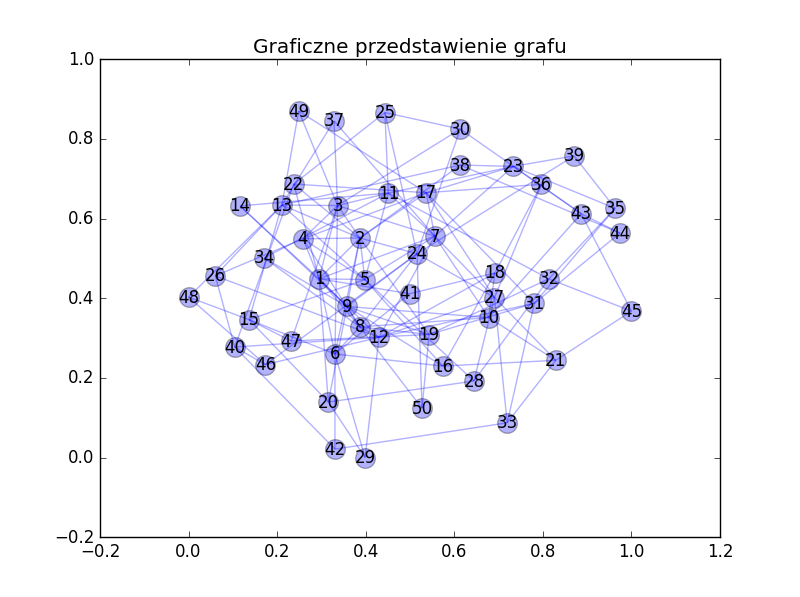
\includegraphics[width=0.8\textwidth]{graf_50.png}
\caption{\small Graf o~50 wierzchołkach}
\label{fig:graf_50}
\end{figure}

\begin{figure}[H]
\centering
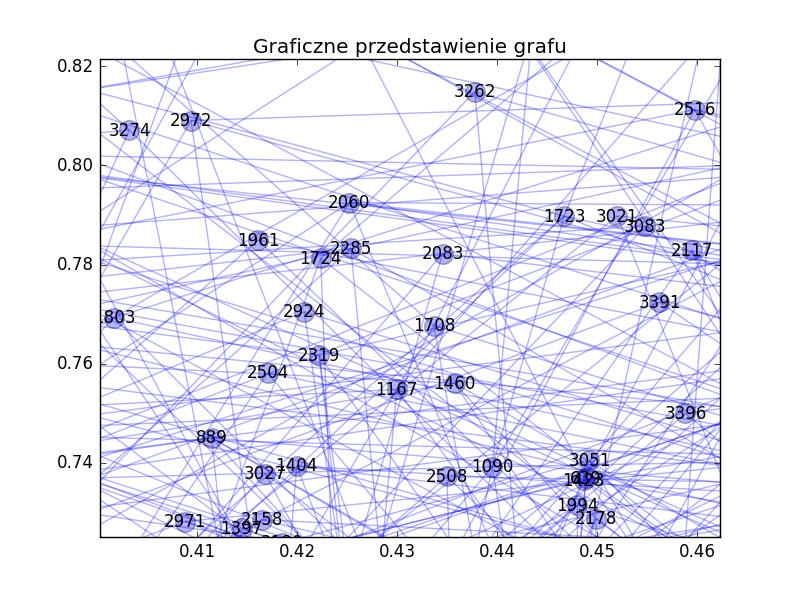
\includegraphics[width=0.8\textwidth]{graf_3400_zoom.png}
\caption{\small Graf o~3400 wierzchołkach --- przybliżenie}
\label{fig:graf_3400_zoom}
\end{figure}

W celu weryfikacji poprawności generowania sieci BA utworzono \textbf{wykresy rozkładów stopni wierzchołków P(k)} dla konkretnej chwili czasowej $t$. Na osi poziomej wykresu oznaczono kolejne wartości stopni wierzchołków. Osi wykresów są przeskalowane do skali \textbf{podwójnie logarytmicznej}. Przedstawiono rozkłady referencyjne wyznaczone teoretycznie zgodnie ze wzorem \ref{eq:roz_ref}:
\begin{equation}
\label{eq:roz_ref}
P(k) = \frac{2 * m^2}{k^3}
\end{equation}

W celu wykazania przybliżonego rozkładu potęgowego $P(k)$ wykreślono na rysunku \ref{fig:rozklad_1} rozkład potęgowy o~współczynniku $\alpha=3$. Badano sieć bezskalową o~parametrach:
\begin{itemize}[nolistsep]
\item $m_0 = 3$
\item $m = 3$
\item $t = 3397$
\end{itemize}

\begin{figure}[H]
\centering
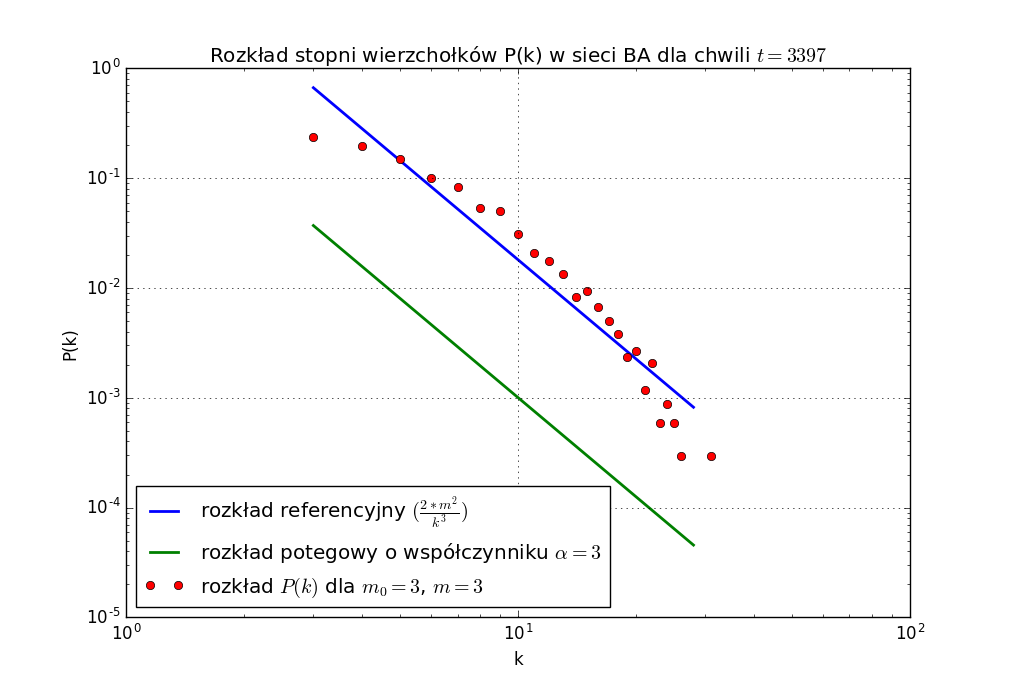
\includegraphics[width=0.8\textwidth]{rozklad_1.png}
\caption{\small Rozkład stopni wierzchołków pojedynczego grafu}
\label{fig:rozklad_1}
\end{figure}

% \noindent
% \begin{minipage}[H]{\textwidth}

Rysunek \ref{fig:rozklad_1} potwierdza \textbf{przybliżony rozkład potęgowy dla wierzchołków}. Stopnie wierzchołków ,,oscylują'' wokół referencyjnego rozkładu. Na rysunkach \ref{fig:rozklad_10}  oraz 
\ref{fig:rozklad_100}  zobrazowano uśrednione rozkłady $P(k)$ z~odpowiednio \textbf{10-ciu i~stu realizacji} sieci bezskalowej generowanej dla identycznych parametrów.

Zbadano również rozkłady dla sieci o~parametrach:

\noindent
\begin{minipage}[H]{0.45\textwidth}
\centering
Rysunek \ref{fig:rozklad_5_1_3397}:
\begin{itemize}[nolistsep]
\item $m_0 = 5$
\item $m = 1$
\item $t = 3395$
\end{itemize}
\end{minipage}
\begin{minipage}[H]{0.45\textwidth}
\centering
Rysunek \ref{fig:rozklad_2_2_198}:
\begin{itemize}[nolistsep]
\item $m_0 = 2$
\item $m = 2$
\item $t = 198$
\end{itemize}
\end{minipage}

% \end{minipage}



\begin{figure}[H]
\centering
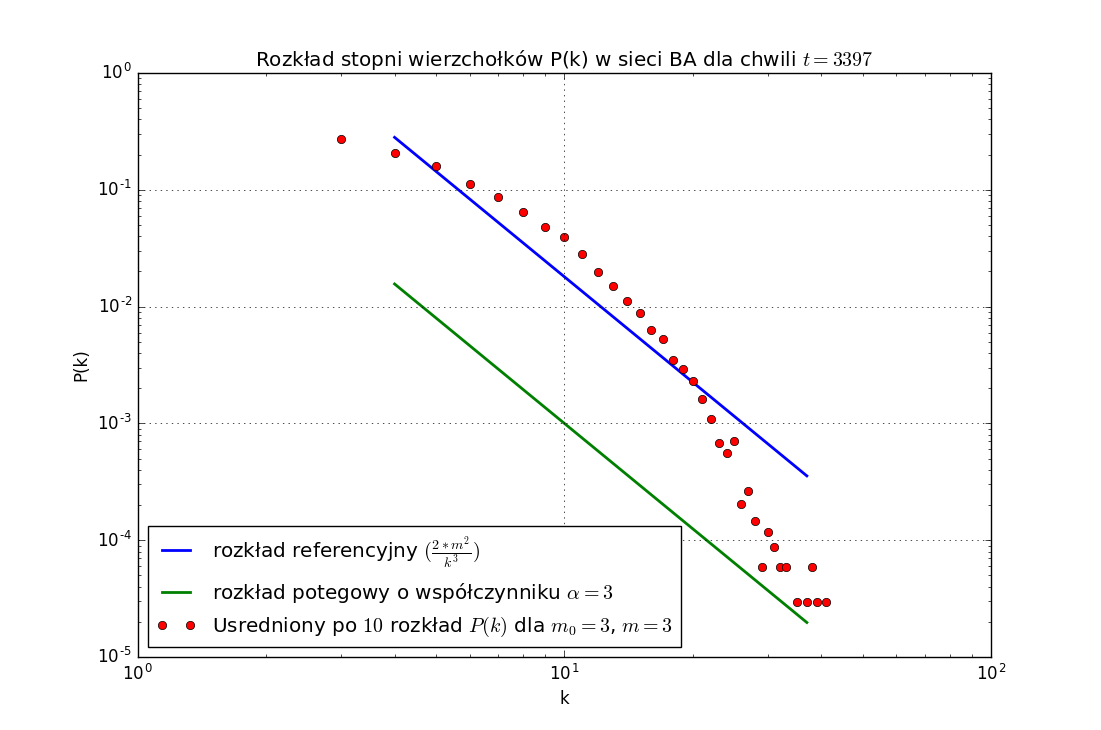
\includegraphics[width=0.8\textwidth]{rozklad_10.png}
\caption{\small Rozkład stopni wierzchołków, uśredniony z~10 prób}
\label{fig:rozklad_10}
\end{figure}

\begin{figure}[H]
\centering
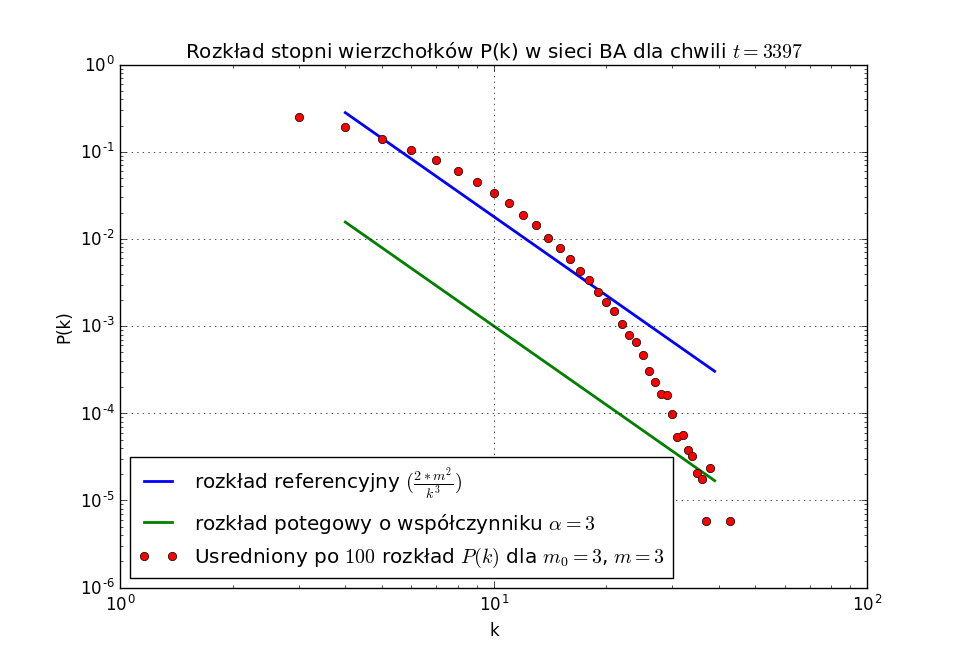
\includegraphics[width=0.8\textwidth]{rozklad_100.png}
\caption{\small Rozkład stopni wierzchołków, uśredniony ze 100 prób}
\label{fig:rozklad_100}
\end{figure}

\begin{figure}[H]
\centering
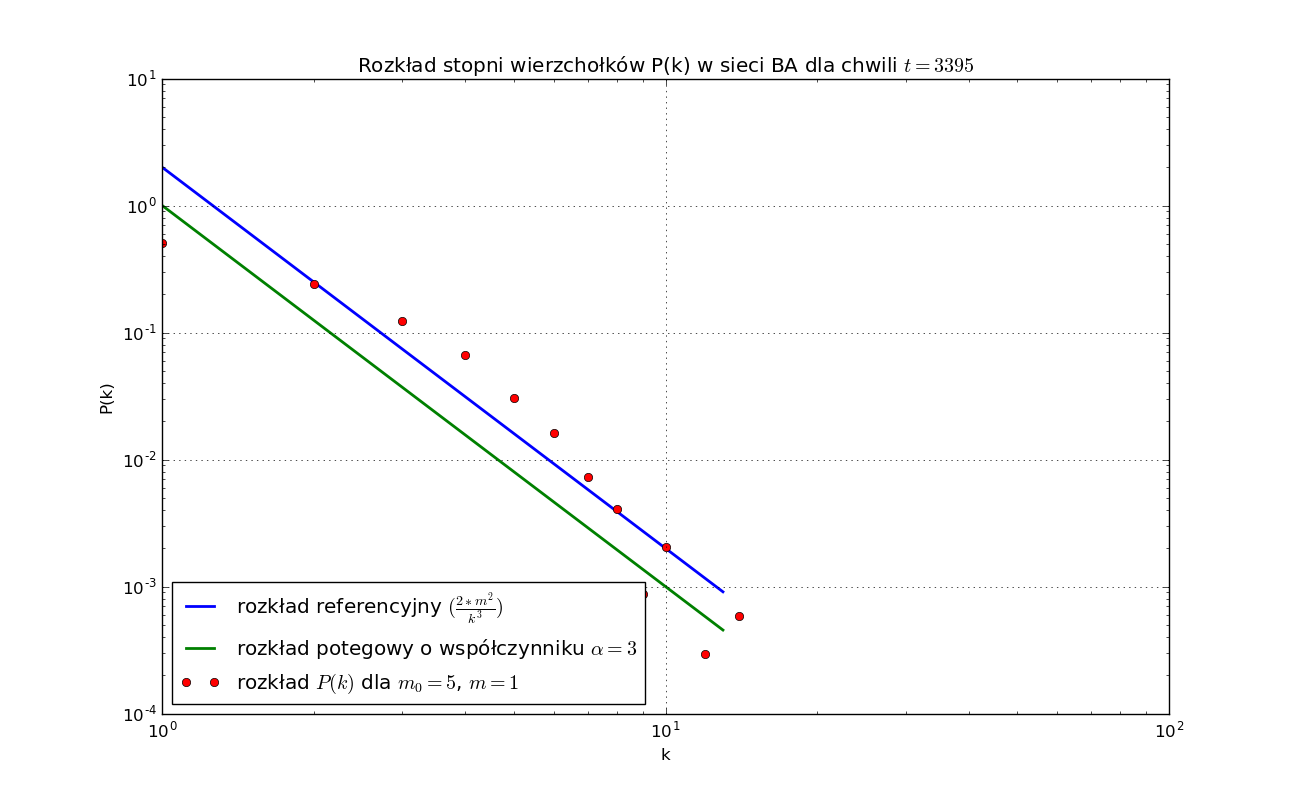
\includegraphics[width=0.8\textwidth]{rozklad_5_1_3397.png}
\caption{\small Rozkład stopni wierzchołków}
\label{fig:rozklad_5_1_3397}
\end{figure}

\begin{figure}[H]
\centering
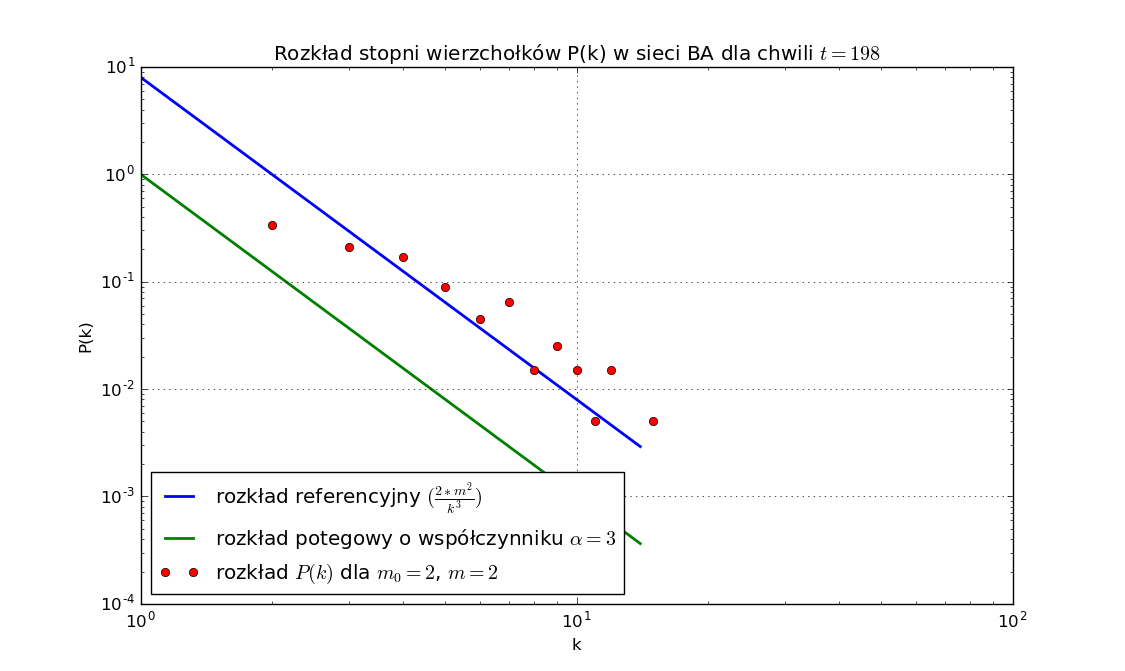
\includegraphics[width=0.8\textwidth]{rozklad_2_2_198.png}
\caption{\small Rozkład stopni wierzchołków}
\label{fig:rozklad_2_2_198}
\end{figure}

\subsection{Propagacja epidemii}
\label{subsec:propagacja_epidemii}

Po wykazaniu poprawności generowanych grafów reprezentujących sieci bezskalowe przystąpiono do realizacji propagacji epidemii. Protokół badań przedstawia się następująco:
\begin{enumerate}
\item Wygeneruj sieć bezskalową o~zadanych parametrach: $m$, $m_0$, $t$.
\item Ustal parametry modelu SIS: $\beta$, $\gamma$, $t_{max}$ - zakończenie symulacji z~tej chwili czasowej, $n_{sim}$ - liczba przeprowadzanych symulacji dla identycznych warunków początkowych (te same zakażone wierzchołki).
\item Zakaź wybrany wierzchołek.
\item Wylicz wektor $i_k(0)$.
\item Wylicz wartość pochodnej dla równania różniczkowego \ref{eq:di_k}. Wylicz wektory $i_k(t)$. dla $t$ dążącego do $t_{max}$
\item Wylicz rozwiązanie równania różniczkowego dla $t$ zbiegającego do nieskończoności.
\item Przeprowadź symulację - wierzchołki ,,zdrowieją'' lub ,,chorują'' z~parametrami odpowiednio $\beta$, $\gamma$.
\item Przeprowadź symulację z~uśrednianiem.
\item Dla zadanego stopnia wierzchołka $k$ wykreśl wykresy przedstawiające zmianę prawdopodobieństwa, że przechowuje on stan ,,chory'' od $t=0$ do $t=t_{max}$.
\end{enumerate}

\subsection{Symulacja dla pierwszej sieci}
\label{subsec:sym_pierwsza_siec}

Dla każdej próby generowano graf od nowa. Dla sieci bezskalowej o~parametrach $m_0 = 3$,$m = 3$,$t = 3397$ na poniższym rysunku \ref{fig:i3_zwykly} wykreślono linią niebieską \textbf{teoretyczną krzywą dla wektora $i_k(t)$} w~kolejnych chwilach czasowych dla wierzchołków w~sieci bezskalowej o~zadanym stopniu $k$. Punktami zaznaczono kolejne wartości otrzymane w~wyniku symulacji epidemii. Przyjęto następujące wartości parametrów dla epidemii:
\begin{itemize}[nolistsep]
\item $k = 3$
\item $t_{max} = 200$
\item $\beta = 0.04$
\item $\gamma = 0.03$
\item $\lambda = 1.33$
\item teoretyczna wartość progu $\lambda_c = 0.167$
\item symulacyjna wartość progu $\lambda_c = 0.174$
\end{itemize}

Na rysunkach \ref{fig:i4_zwykly}, \ref{fig:i5_zwykly} oraz \ref{fig:i6_zwykly} wykreślono prawdopodobieństwa infekcji dla wierzchołków o~stopniach odpowiednio: $k=4,5,6$.

\begin{figure}
\centering
\begin{minipage}[H]{0.45\textwidth}
  \centering
  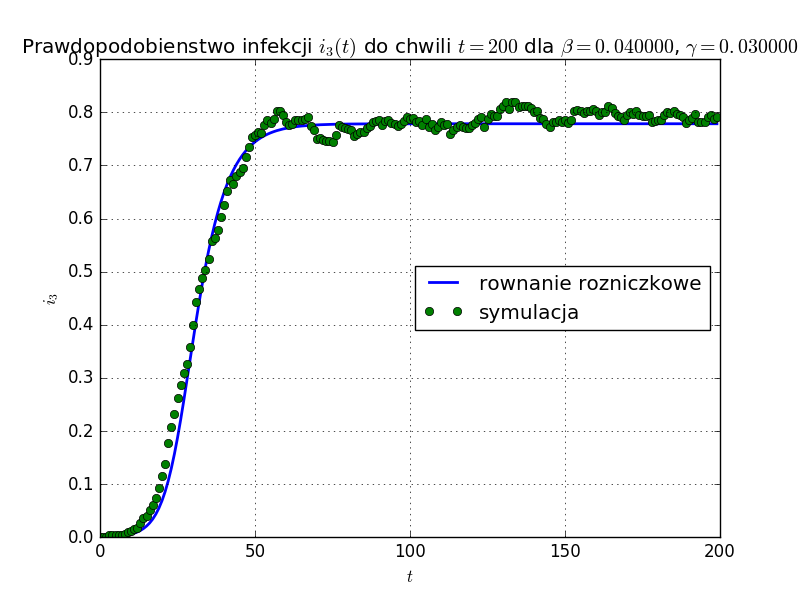
\includegraphics[width=0.8\textwidth]{i3_zwykly.png}
  \caption{\small Propagacja infekcji dla \\ wierzchołków o~stopniu $k=3$}
  \label{fig:i3_zwykly}
\end{minipage} 
\begin{minipage}[H]{0.45\textwidth}
  \centering
  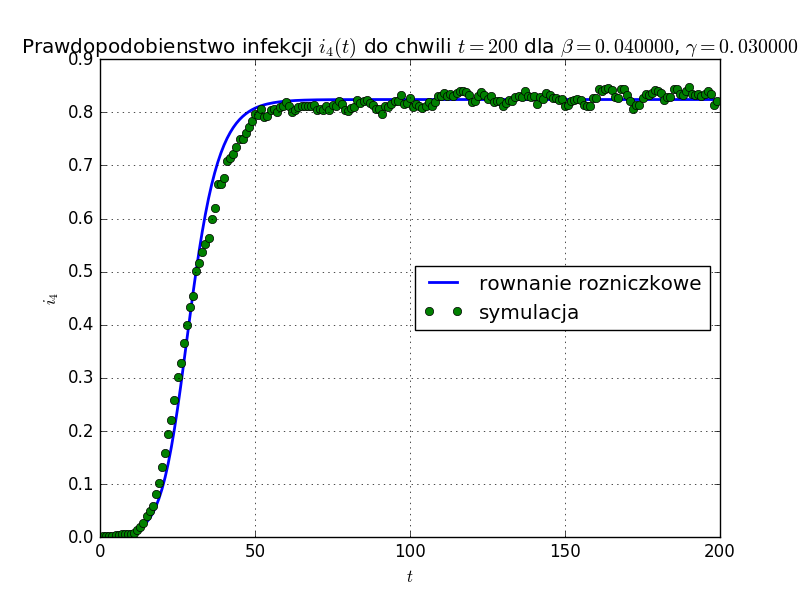
\includegraphics[width=0.8\textwidth]{i4_zwykly.png}
  \caption{\small Propagacja infekcji dla \\ wierzchołków o~stopniu $k=4$}
  \label{fig:i4_zwykly}
\end{minipage} 
\begin{minipage}[H]{0.45\textwidth}
  \centering
  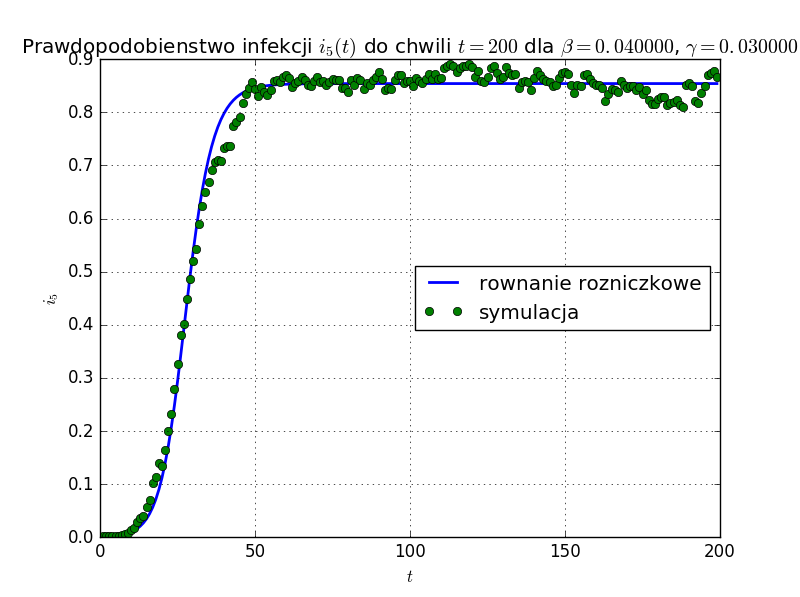
\includegraphics[width=0.8\textwidth]{i5_zwykly.png}
  \caption{\small Propagacja infekcji dla \\ wierzchołków o~stopniu $k=5$}
  \label{fig:i5_zwykly}
\end{minipage}
\begin{minipage}[ht]{0.45\textwidth}
  \centering
  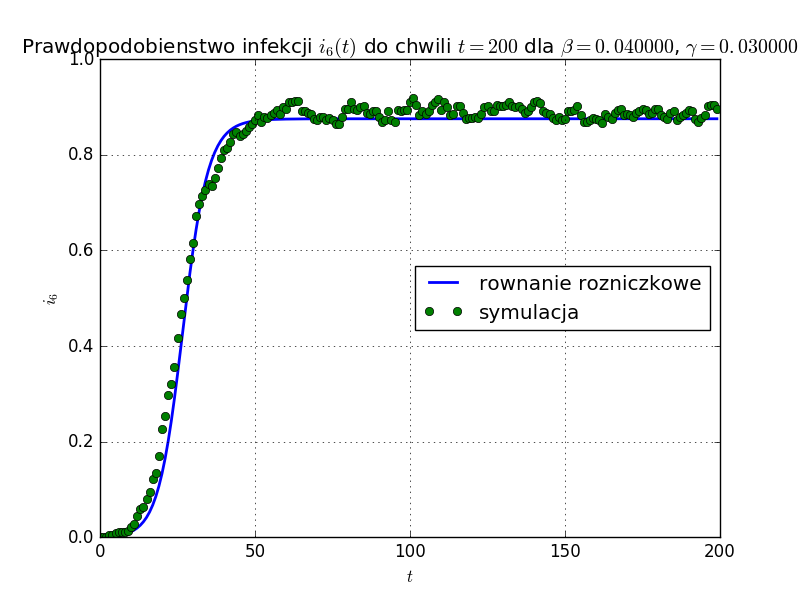
\includegraphics[width=0.8\textwidth]{i6_zwykly.png}
  \caption{\small Propagacja infekcji dla \\ wierzchołków o~stopniu $k=6$}
  \label{fig:i6_zwykly}
\end{minipage}
\end{figure}

% MD: Z~punktu badawczego myślę, ze mało istotne jest to uśrednianie
% \textbf{\textcolor{red}{TODO}}
% \textcolor{red}{komentarz: obrazki --- propagacja}
% \textcolor{red}{przesunięcie wykresu}
% \textcolor{red}{uśrednienie}

Następnie przeprowadzono symulację dla tej samej sieci bezskalowej, dla której współczynnik zakażania jest równy współczynnikowi zdrowienia. Wyniki przedstawiono na rysunku \ref{fig:symulacja_003_003.png}.
\begin{itemize}[nolistsep]
\item $k = 10$
\item $t_{max} = 200$
\item $\beta = 0.03$
\item $\gamma = 0.03$
\item $\lambda = 1.0$
\item teoretyczna wartość progu $\lambda_c = 0.166$
\item symulacyjna wartość progu $\lambda_c = 0.191$
\end{itemize}

\begin{figure}[H]
\centering
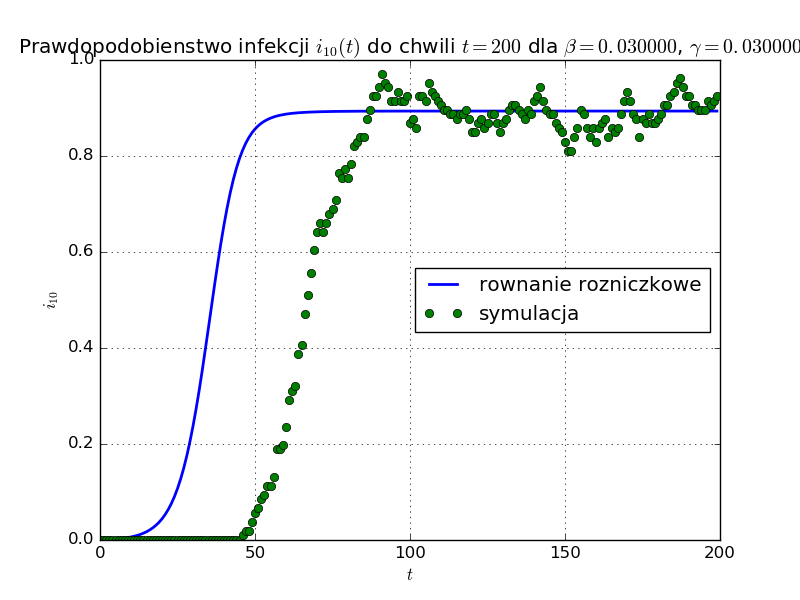
\includegraphics[width=0.8\textwidth]{symulacja_003_003.png}
\caption{\small Propagacja infekcji dla wierzchołków o~stopniu $k=10$}
\label{fig:symulacja_003_003.png}
\end{figure}

Symulacja z~pewnym opóźnieniem w~stosunku do teoretycznego przebiegu ustala się na spodziewanym poziomie.

Kolejnym krokiem było zwiększenie wartości prawdopodobieństwa, że dany osobnik populacji wyzdrowieje (Rysunek \ref{fig:symulacja_003_015.png}).
\begin{itemize}[nolistsep]
\item $k = 6$
\item $t_{max} = 200$
\item $\beta = 0.03$
\item $\gamma = 0.15$
\item $\lambda = 0.2$
\item teoretyczna wartość progu $\lambda_c = 0.166$
\item symulacyjna wartość progu $\lambda_c = 0.178$
\end{itemize}

\begin{figure}[H]
\centering
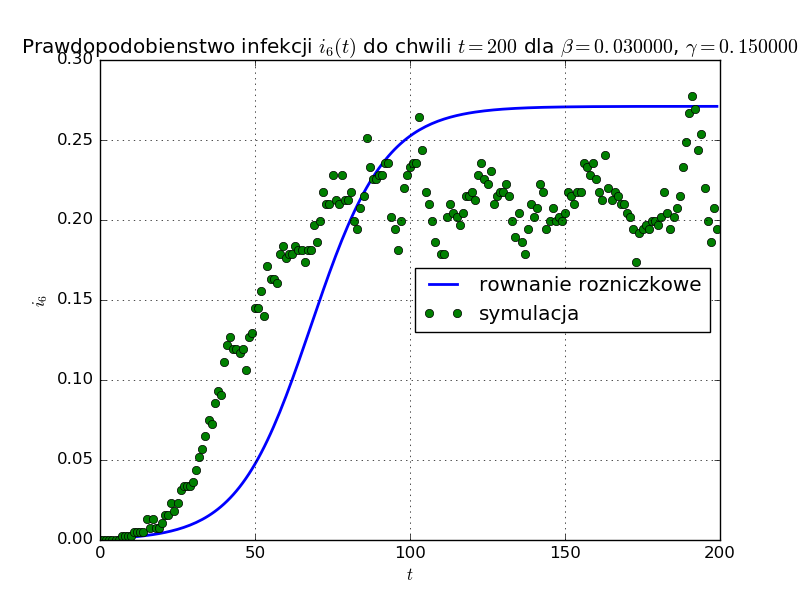
\includegraphics[width=0.8\textwidth]{symulacja_003_015.png}
\caption{\small Propagacja infekcji dla wierzchołków o~stopniu $k=6$}
\label{fig:symulacja_003_015.png}
\end{figure}

Drastyczne zdrowienie osobników populacji pozwala na stłumienie epidemii (Rysunek \ref{fig:symulacja_003_055.png}. Dla tego przykładu wartość $\lambda < \lambda_c$. Przyjęte wartości parametrów:
\begin{itemize}[nolistsep]
\item $k = 6$
\item $t_{max} = 200$
\item $\beta = 0.03$
\item $\gamma = 0.55$
\item \textbf{$\lambda = 0.05$}
\item teoretyczna wartość progu $\lambda_c = 0.166$
\item symulacyjna wartość progu $\lambda_c = 0.190$
\end{itemize}

Na koniec należy zauważyć, że w~niektórych (nielicznych) symulacjach prawdopodobieństwo infekcji było prawie przez całą symulację stałe, równe 0 (rysunek \ref{fig:i3_00}). Jest to przypadek szczególny, omówiony zostanie w~rozdziale \ref{sec:wnioski}.

\begin{figure}[H]
\centering
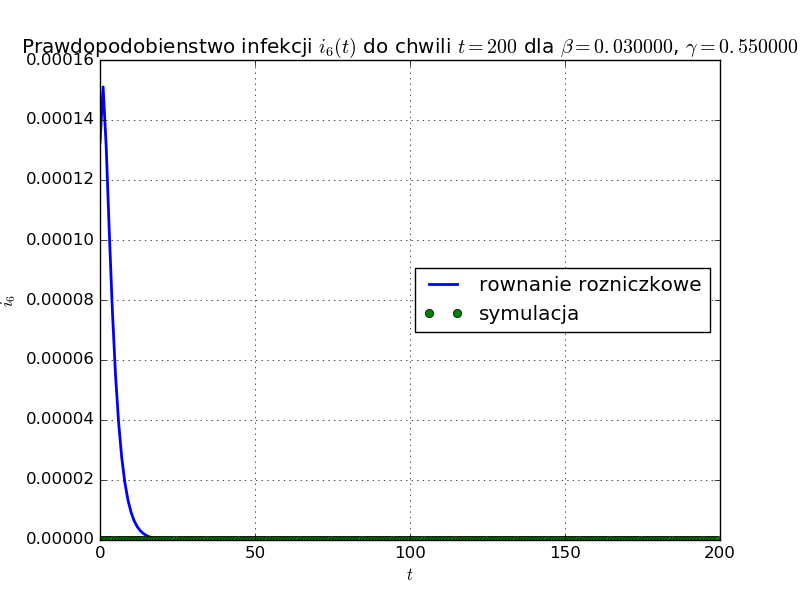
\includegraphics[width=0.8\textwidth]{symulacja_003_055.png}
\caption{\small Propagacja infekcji dla wierzchołków o~stopniu $k=6$}
\label{fig:symulacja_003_055.png}
\end{figure}

\begin{figure}[H]
\centering
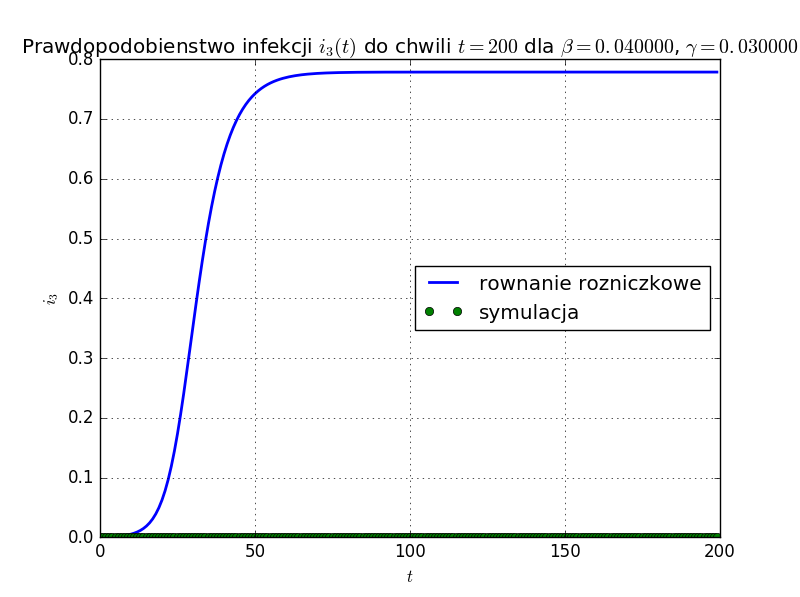
\includegraphics[width=0.8\textwidth]{i3_00.png}
\caption{\small Szczególny przypadek wygaśnięcia epidemii}
\label{fig:i3_00}
\end{figure}

\subsection{Symulacja dla drugiej sieci}
\label{subsec:sym_druga_siec}

Następną symulację epidemii przeprowadzono dla sieci bezskalowej o~parametrach $m_0 = 3$,$m = 1$,$t = 997$. Sieć ta ma strukturę bardzo zbliżoną do drzewa --- ale nim nie jest, ponieważ zawiera jedną klikę (początkowy graf). Dla każdej próby generowano graf od nowa. Przyjęto następujące wartości parametrów dla epidemii:
\begin{itemize}[nolistsep]
\item $k = 4$
\item $t_{max} = 800$
\item $\beta = 0.14$
\item $\gamma = 0.15$
\item $\lambda = 0.93$
\item teoretyczna wartość progu $\lambda_c = 0.493$
\item symulacyjna wartość progu $\lambda_c = 0.499$
\end{itemize}

\begin{figure}[H]
\centering
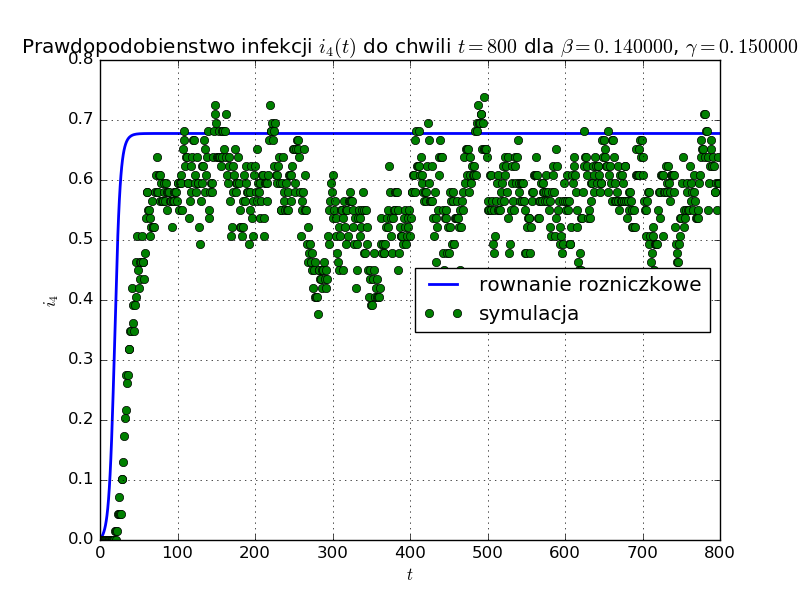
\includegraphics[width=0.8\textwidth]{symulacja_014_015_tree.png}
\caption{\small Propagacja infekcji dla wierzchołków o~stopniu $k=4$}
\label{fig:symulacja_014_015_tree}
\end{figure}

W czasie niektórych symulacji chorzy zdrowieli wyjątkowo szybko, co powodowało, że epidemia była tłumiona już we wczesnym stadium (jak w~przypadku pierwszej sieci, sekcja \ref{subsec:sym_pierwsza_siec}). Rysunek \ref{fig:sym_drzewo} ukazuje próbę, w~której epidemia rozpropagowała się.

Kolejną symulację przeprowadzono dla sieci bezskalowej o~tych samych parametrach ($m_0 = 3$,$m = 1$,$t = 997$). Dla tego przypadku wartość $\lambda < \lambda_c$. Przyjęto następujące wartości parametrów dla epidemii:
\begin{itemize}[nolistsep]
\item $k = 4$
\item $t_{max} = 800$
\item $\beta = 0.14$
\item $\gamma = 0.65$
\item \textbf{$\lambda = 0.21$}
\item teoretyczna wartość progu $\lambda_c = 0.493$
\item symulacyjna wartość progu $\lambda_c = 0.500$
\end{itemize}

\begin{figure}[H]
\centering
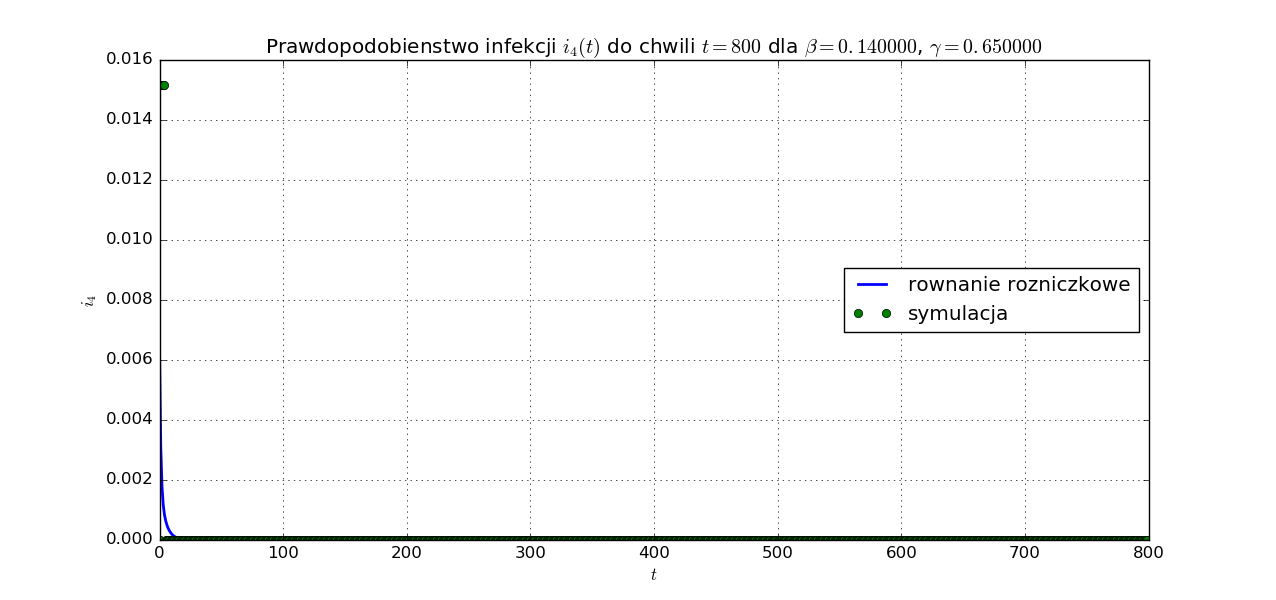
\includegraphics[width=0.8\textwidth]{symulacja_014_065_tree_2.png}
\caption{\small Propagacja infekcji dla wierzchołków o~stopniu $k=4$}
\label{fig:symulacja_014_065_tree}
\end{figure}

Początkowe prawdopodobieństwo zakażenia $i_k$ zostało szybko zredukowane. Wyniki pokrywają się z~krzywą wyznaczoną teoretycznie.


\section{Wnioski}
\label{sec:wnioski}

Zaimplementowanie rozwiązanie do propagacji epidemii dla populacji modelowanej przez sieci bezskalowe działa poprawnie. Sprawdzono różne konfiguracje sieci bezskalowych oraz zbadano ich rozkłady stopni wierzchołków. Wykazano, że w~przybliżeniu realizują one teoretyczny rozkład dany wzorem. 

\subsection{Współczynniki}
\label{subsec:wnioski_wspolczynniki}

Zachowanie sieci zależne jest od współczynników określających prawdopodobieństwo zakażenia się od sąsiada ($\pmb{\beta}$) oraz prawdopodobieństwo wyzdrowienia ($\pmb{\gamma}$). Ustala się je na początku symulacji. W~celu zbadania epidemii przeprowadzono symulacje dla różnych ich wartości. Dowiedziono, że dla sieci bezskalowych trudno jest powstrzymać propagację chorób i~dla późnych chwil czasowych ustala się ona na konkretnym poziomie powodując pandemię. Dzieje się tak, ponieważ:
\begin{enumerate}[label=\arabic*), nolistsep]
\item Teoria (sekcja \ref{subsec:zalozenia_modelu_sis}: założenia i~sekcja \ref{subsec:rownania_rozniczkowe_opisujace_model}: równanie \ref{eq:lambda_c}) mówi, że zjawisko to ma miejsce, jeżeli \[ \lambda>\lambda_c\] gdzie: \[ \lambda = \frac{\beta}{\gamma} \land \lambda_c = \frac{\langle k \rangle}{\langle k^2 \rangle} \]
\item W sieciach bezskalowych współczynnik $\lambda_c$ jest bardzo niski, ze względu na ich charakter --- a~w~szczególności występowanie wierzchołków wysokiego stopnia.
\end{enumerate}
Spostrzeżenia dotyczące współczynnika $\lambda$:
\begin{enumerate}[label=\arabic*), nolistsep]
\item Jeżeli $\lambda > \lambda_c$, epidemia rozwinie się i~ustali na konkretnym poziomie, przekształcając się w~pandemię (np. rysunki \ref{fig:i3_zwykly}-\ref{fig:i6_zwykly}).
\item Im współczynnik $\lambda$ jest wyższy, tym szybciej propaguje epidemia.
  \begin{itemize}
  \item Dla niskich $\lambda$, jednak ciągle wyższych od $\lambda_c$, można zaobserwować przesunięcie wykresu wzdłuż osi czasu (OX) w~prawo (w kierunku wyższych wartości) oraz zwiększone pochylenie. To oznacza, że choroba wolniej zajmuje nowe wierzchołki na początku (rysunek \ref{fig:symulacja_003_015.png}). 
  \end{itemize}
\item Gdy $\lambda \rightarrow \lambda_c^+$, epidemia wprawdzie dąży do pandemii, jednak dużo mniej stabilnie i~zdecydowanie wolniej. Rozwój epidemii jest na początku tłumiony (rysunek \ref{fig:symulacja_003_015.png}).
\item Jeżeli $\lambda < \lambda_c$, epidemia wygaśnie (rysunek \ref{fig:symulacja_003_055.png}),
  \begin{itemize}
  \item Tym szybciej, im niższy współczynnik $\lambda$
  \item Zwiększanie współczynnika wyzdrowienia ($\gamma$) w~stosunku do zachorowania ($\beta$) (poprzez działania prewencyjne, profilaktyczne itd.) pozwala stłumić propagację choroby już we wczesnym stadium,
  \item Należy jednak mieć na uwadze, że stan taki w~sieciach bezskalowych występuje dosyć rzadko.
  \end{itemize}
\end{enumerate}

\subsection{Symulacja grafowa a~rozwiązanie teoretyczne}
\label{subsec:wnioski_sym_a_teo}

Różnice w~ilości zakażonych w~rozwiązaniu teoretycznym i~symulacji grafowej wynikają przede wszystkim z tego, że:
\begin{enumerate}[label=\arabic*), nolistsep]
\item W~rozwiązaniu teoretycznym operujemy prawdopodobieństwami i~modelujemy rozkład prawdopodobieństwa, niezależny od losowych zmian w grafie,
\item W~symulacji zliczamy wierzchołki (stosunek liczby zakażonych do całkowitej ich liczby), których stany są zależne od losowych zmian w grafie.
\end{enumerate}

Zdarza się, że epidemia wygasa na samym początku symulacji  (rysunek \ref{fig:i3_00}. W~takiej sytuacji, wynik symulacji będzie całkowicie niezgodny z~rozwiązaniem teoretycznym. Dzieje się tak, ponieważ:
\begin{enumerate}[label=\arabic*), nolistsep]
\item Stosowany jest tutaj losowy algorytm grafowy, każdy wierzchołek zmienia swój stan z
~określonym prawdopodobieństwem, 
\item Do zakażenia potrzebny jest kontakt osobnika zakażonego ze zdrowym, czyli musi istnieć osobnik zakażony (musi istnieć wierzchołek w~stanie I, mający krawędź do wierzchołka w~stanie S),
\item Do wyzdrowienia potrzebny jest jedynie osobnik zakażony (wierzchołek w~stanie I)
\item Jeżeli zdarzy się tak, że pacjent zero wyzdrowieje na samym początku, jedyny wierzchołek o~stanie I~zmieni stan na S~--- w~sieci pozostaną jedynie wierzchołki w~stanie S), epidemia wygaśnie na samym początku i~nie będzie miała jak się rozwinąć. 
\end{enumerate}
\par
Niezależnie od współczynników, ze względu na losowość zmian stanów wierzchołków i~połączeń (np. początek epidemii wśród wierzchołków niskiego stopnia --- utrudnione warunki jej rozwoju), epidemia może w~początkowej fazie nie rozprzestrzeniać się z~dużą prędkością (rysunek \ref{fig:symulacja_003_003.png}), ale przyspieszyć kilka momentów $t$~później. Obserwujemy wtedy znaczne przesunięcie fazy gwałtownego wzrostu epidemii dla symulacji grafowej i~teoretycznego rozwiązania różniczkowego.
\par
W~drugiej badanej sieci można zaobserwować wolniejszą i~mniej stabilną propagację (rysunek \ref{fig:symulacja_014_015_tree}), choć ostatecznie wynik też ustala się na określonym poziomie. Dzieje się tak, ponieważ druga sieć ma mniej krawędzi (nowe wierzchołki tworzą po jednej krawędzi zamiast trzech --- jak w~ pierwszej sieci), co przekłada się na mniejszą ogólną liczbę połączeń. To z~kolei (w~rzeczywistości) oznacza mniej rozbudowaną sieć kontaktów między ludźmi, a~więc mniejsze możliwości rozprzestrzeniania się choroby. 


% \textbf{\textcolor{red}{Co z~uśrednianiem?}}

\end{enumerate}

\clearpage
%*******************************************************************************
% Bibliografia - spis literatury wykorzystanej przy tworzeniu pracy
%*******************************************************************************
%\clearpage
\begin{thebibliography}{99}
\addcontentsline{toc}{chapter}{Bibliografia}

%1
\bibitem{SieciZlozone} Fronczak Agata, Fronczak Piotr: \emph{,,Świat sieci złożonych''}, 
\newline Wyd. I, Warszawa, wyd. PWN, 2009, ISBN: 978-83-01-15987-0.

%2
\bibitem{EpiWSieciach} Fronczak Agata, Fronczak Piotr: \emph{,,Epidemie w sieciach złożonych''} [online],  \\ 28.10.2010,
\url{ http://www.if.pw.edu.pl/~agatka/moodle/epidemie.html } , \\ dostęp: 20.11.2016r.



\end{thebibliography}

\clearpage

%===============================================================================


\end{document}